%% content.tex
%%

%% ===========================
\chapter{Systemanalyse}
\label{ch:Systemanalyse}
%% ===========================

Zu Beginn der Arbeiten wird eine Systemanalyse zur Ermittlung des Ist- und Sollzustandes durchgeführt. Nach \cite{SWB-380277719} versteht man darunter das Beschreiben der vorhandenen und zukünftigen Systeme. Zuerst wird in Abschnitt \ref{ch:Systemanalyse:sec:genesisWorld} eine Ist-Analyse durchgeführt. In Abschnitt \ref{ch:Systemanalyse:sec:Anforderungsanalyse} wird auf die, an das System gestellt, Anforderungen eingegangen. Aufbauend auf den Anforderungen werden in Abschnitt \ref{ch:Systemanalyse:sec:Information} die relevanten Daten für die Umsetzung ermittelt. 

%% ===========================
\section{CAS genesisWorld}
\label{ch:Systemanalyse:sec:genesisWorld}
%% ===========================

CAS genesisWorld ist eine Software, die Organisation und Zusammenarbeit in Kundenbeziehungen und zwischen Kollegen steigern soll. Alle Informationen bzw. Daten werden in CAS genesisWorld zentral gespeichert und sind so für alle verfügbar. Welche Daten ein Anwender sieht, hängt von seinen Rechten und Einstellungen ab. Die Daten, d.h. Termine, Aufgaben, Adressen, Dokumente usw. werden in CAS genesisWorld von den Nutzern gepflegt und aktuell gehalten. Darüber hinaus lassen sich wie in Abbildung \ref{picGwCon} dargestellt, alle Daten beliebig miteinander verknüpfen. So werden zusätzliche Zusammenhänge deutlich und der Informationsgehalt steigt. Ein Besprechungstermin lässt sich beispielsweise mit den Adressen der Teilnehmer und dem Dokument der Tagesordnung verknüpfen.

\begin{figure}[H]
	\centering
  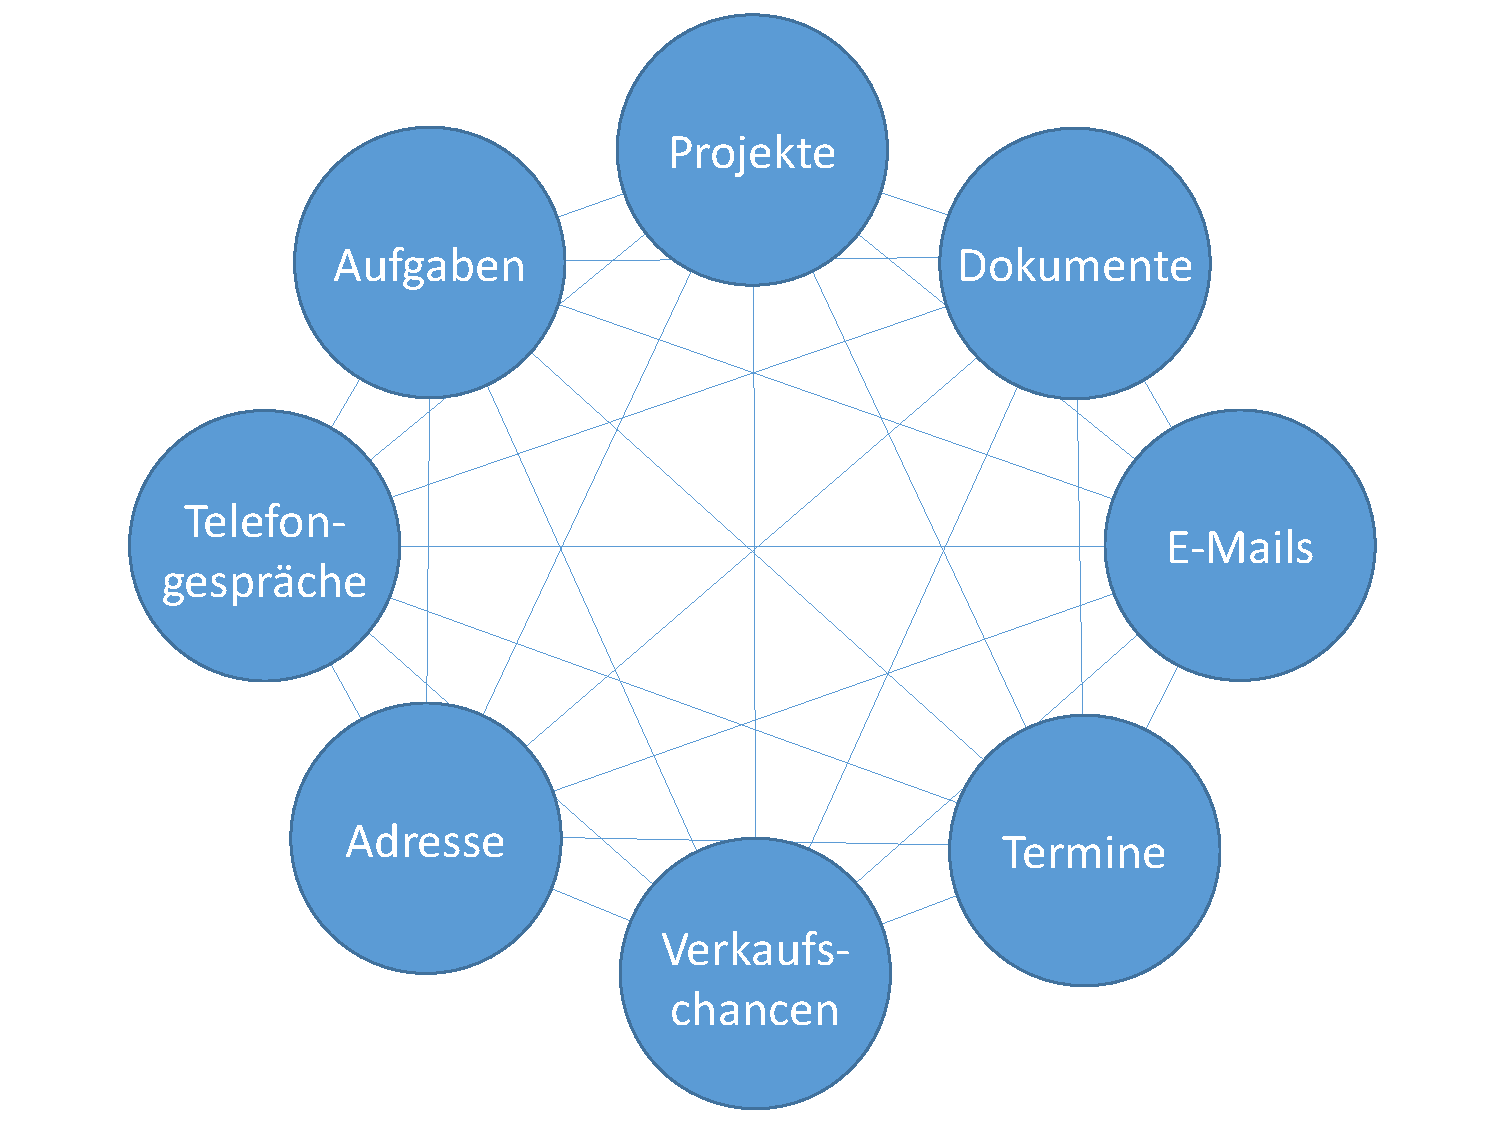
\includegraphics[width=0.5\textwidth, width=0.5\textwidth]{pics/CAS_connections.pdf}
	\caption{Verknüpfungen in CAS genesisWorld}
	\label{picGwCon}
\end{figure}

%% ===========================
\subsection{Architektur}
%% ===========================

Die N-Tier-Architektur von CAS genesisWorld lässt sich in drei wesentliche Bereiche gliedern:

\begin{itemize}

	\item Die Präsentationsclients umfassen alle Dienste, die Informationen in Bildschirmansichten den Benutzern zur Verfügung stellen.
	
	\item Der Applikationsserver umfasst alle Dienste, um die Geschäftslogik zu kapseln, Änderungen zu protokollieren, Benutzerrechte zu prüfen und die aufbereiteten Informationen den Präsentationsdiensten zur Verfügung zu stellen.
	
	\item Die Datenbankschicht umfasst alle Dienste die zur Datenhaltung selbst notwendig sind.
\end{itemize}


%% ===========================
\subsection{Präsentationsschicht \& Logikschicht}
%% ===========================

Der CAS genesisWorld Client existiert in Form einer Windowsanwendung, als mobile Version in Android, Windows Phone, BlackBerry OS und iOS. Die Kommunikation der Clients mit CAS genesisWorld findet über das REST-Protokoll statt \cite{cas2013a}.

Die Funktionalität des CAS genesisWorld Anwendungsservers wurde in Form von COM-Objekten implementiert. Damit stehen dessen Dienste auch Dritten zur Verfügung, die dadurch mit eigenen Applikationen die Informationen von CAS genesisWorld präsentieren oder weiterverarbeiten können. Eine erster Überblick der CAS genesisWorld Komponenten ist in Abbildung \ref{gw_Architektur} zu sehen. Als Basisdienste stehen der UserService und der DataService zu Verfügung. Für die Anmeldung und Rechteverwaltung ist der UserService zuständig. Der DataService ist als zentraler Dienst für den Zugriff auf die CAS genesisWorld Daten verantwortlich. Die Schnittstelle des DataService wurde an Microsoft ADO angelehnt. Auf den Basisdiensten aufbauend existieren die Geschäftsdienste, in Form der Schnittstellen der BusinessServices. Diese bieten spezielle Funktionen zu den jeweiligen Anwendungsbereichen.

\begin{figure}[H]
	\centering
  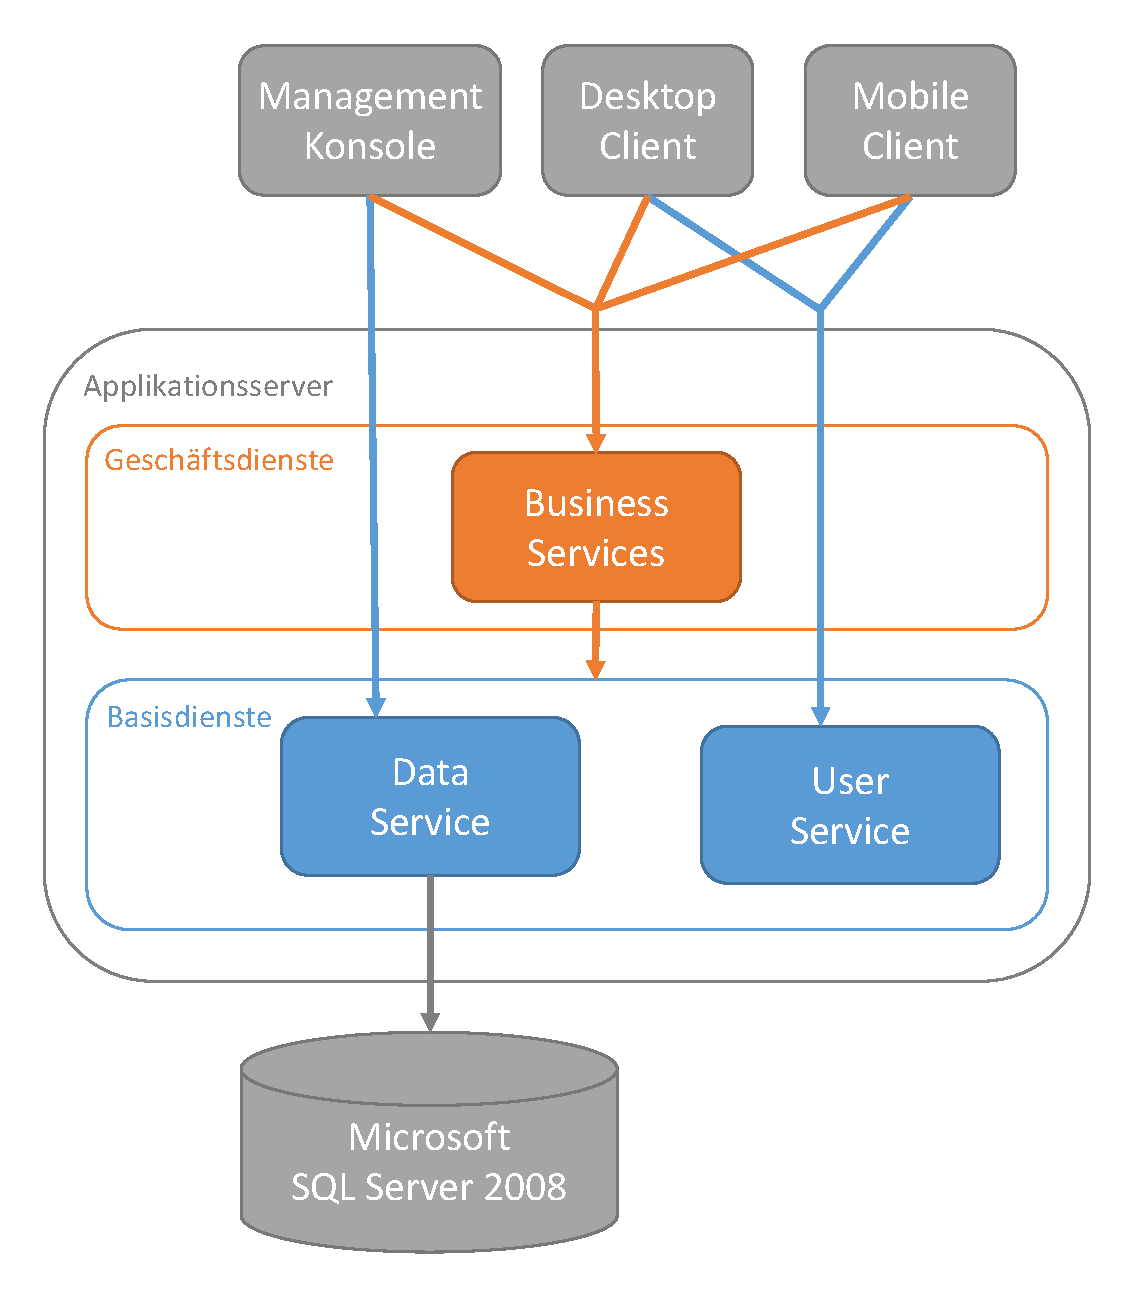
\includegraphics[width=0.6\textwidth, width=0.6\textwidth]{pics/GenesisWorld_Architektur.pdf}
	\caption{Schematische Darstellung der Architektur von CAS genesisWorld}
	\label{gw_Architektur}
\end{figure}

%% ===========================
\subsection{Datenhaltungsschicht}
\label{ch:Systemanalyse:sec:genesisWorld:subsec:db}
%% ===========================

Die Datenhaltungsschicht enthält einen Microsoft SQL Server 2008 (MSSQL). Der SQL Server ist ein relationales Datenbankmanagementsystem (RDBMS) von Microsoft, dass für den Einsatz im Konzernumfeld konzipiert wurde. MSSQL verwendet T-SQL (Transact-SQL), eine Erweiterungen von Sybase und Microsoft, die den SQL-Standard um prozedurale Sprachelemente erweitert \cite{tech2013}. Weiterhin unterstützt MSSQL standardisierte Datenbankschnittstellen, wie Open Database Connectivity (ODBC) und Java Database Connectivity (JDBC).

Beim Schema der Datenbank wird auf eine Besonderheit eingegangen. In relationalen Datenbanken werden Beziehungen über Primär- und Fremdschlüssel abgebildet. Dies ist auch in der MSSQL-Datenbank der Fall, jedoch mit einer Besonderheit. In der MSSQL-Datenbank werden nur Primärschlüssel deklariert. Es werden Fremdschlüssel verwendet allerdings sind sie nicht als solche deklariert.

Ein Grund dafür ist die Art wie die Funktionalität in der Datenbank umgesetzt wurde, die eine Verknüpfung sämtlicher CRM-Objekte ermöglicht. Abbildung \ref{gw_2} zeigt das ER-Modell für die Funktionalität. Bei 398 Tabellen existieren durch die Funktionalität sehr viele M:N-Beziehungen. Anstatt für jede M:N-Beziehung eine separate Tabelle anzulegen wurde lediglich eine Tabelle verwendet. Sie besitzt vier relevante Spalten. In zwei von ihnen werden die Fremdschlüssel der in Beziehung zu setzenden Tabellen aufbewahrt. Damit die nächst höhere Schicht die Fremdschlüssel den entsprechenden Tabellen zuordnen kann werden in den anderen beiden Spalten die Zuordnungskürzel hinterlegt. Jede Tabelle besitzt sein eigenes eindeutiges Kürzel. Die Nutzung einer Auflösungstabelle ist nur möglich weil die beiden Spalten in denen die Fremdschlüssel aufbewahrt werden nicht als solche deklariert sind.

Weiterführende Erläuterungen zum relevanten Teil des Schemas werden in Abschnitt \ref{ch:Systemanalyse:sec:Information} behandelt.

\begin{figure}[ht]
	\centering
  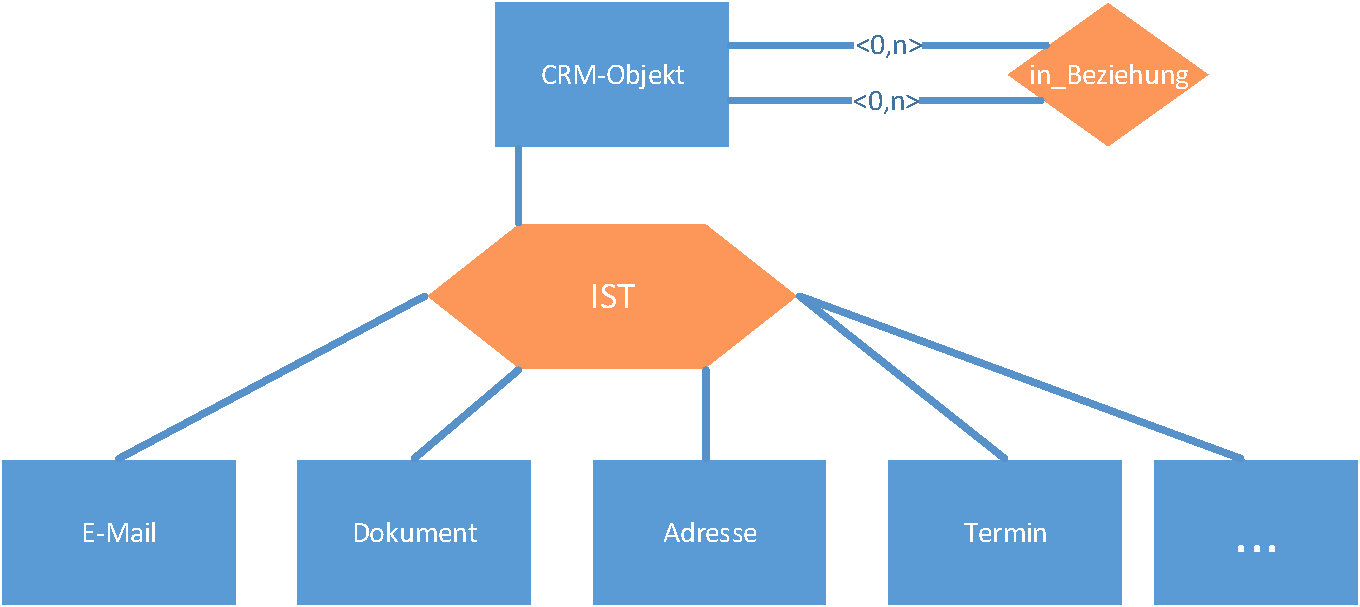
\includegraphics[width=0.9\textwidth, width=0.9\textwidth]{pics/erm.pdf}
	\caption{ER-Modell}
	\label{gw_2}
\end{figure}

Die Spalten \textit{GUID1} und \textit{GUID2} beinhalten die jeweiligen Primärschlüssel der in Beziehung zu setzenden Tabellen. Mithilfe der Spalten \textit{TableSign1} und \textit{TableSign2} können die \textit{GGUID}s den Tabellen, aus denen sie entstammen, zugeordnet werden. Die \textit{GGUID} ist in der gesamten Datenbank eindeutig und dient als Primärschlüssel für jede Tupel in der Datenbank.

%% ===========================
\subsection{Server-SDK-Plugin}
\label{ch:Systemanalyse:sec:genesisWorld:subsec:plugin}
%% ===========================

Die Server-SDK-Plugins bieten die Möglichkeit die Datenverarbeitung, um eine eigene Logik zu erweitern oder zu modifizieren. 

Realisiert werden die Plugins als COM-Objekte, die ein Plugin-Interface namens \textit{IGWSDKDataPlugIn} implementieren. Das erstellte COM-Objekt wird im Server von CASgenesisWorld registriert. Der Server delegiert bei einer Datenoperation den Aufruf an die für den jeweiligen Datensatztypen registrierten Plugins. In Abbildung \ref{gw_plugin} ist ein Beispiel des Vorgangs dargestellt. Die CASTable ist für die Delegation der Datenmanipulation-Anweisungen zuständig. Sie empfängt Anweisungen vom DataService und führt diese auf dem MSSQL-Server aus. Außerdem besitzt sie mit dem Plugin-Direktor eine Komponente mit der Plugins über Änderungen in den Datensätzen informiert werden. Wie in der Abbildung zu sehen werden zuerst die fest integrierten Plugins wie das CAS-Address-Plugin benachrichtigt. Anschließend werden die von Dritten erstellten Plugins informiert.

\begin{figure}[H]
	\centering
  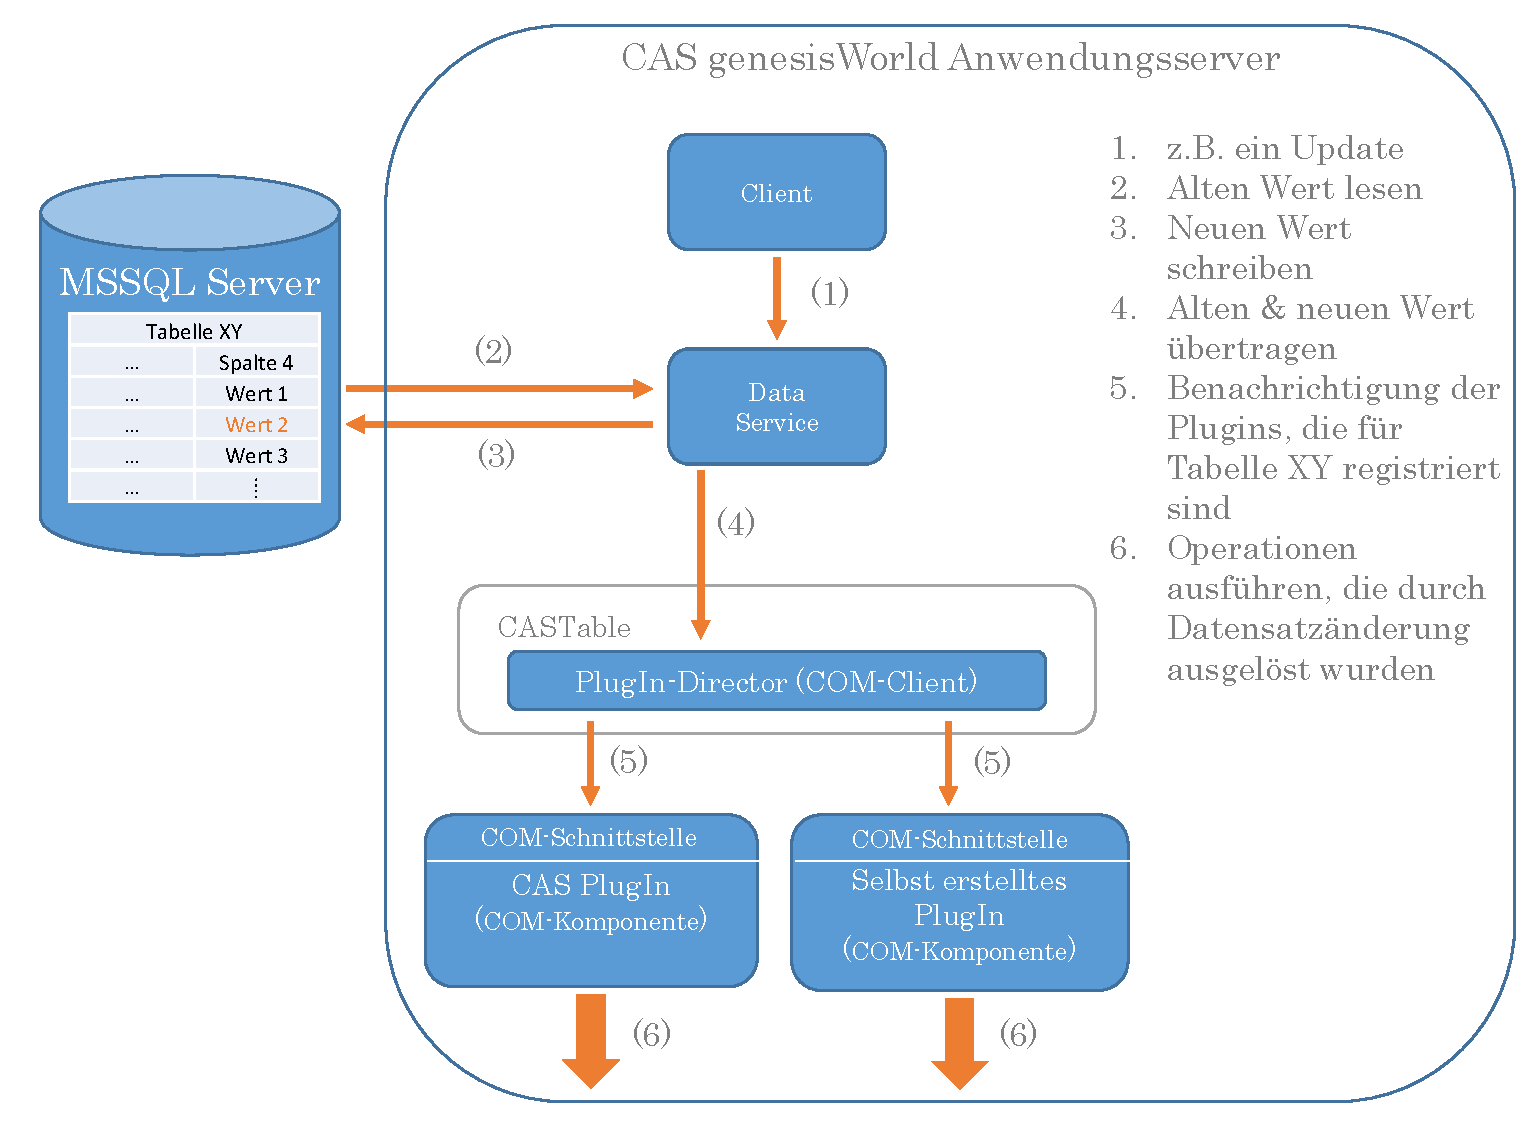
\includegraphics[width=1.0\textwidth, width=1.0\textwidth]{pics/analyse_plugins.pdf}
	\caption{Beispiel zur Benachrichtigung von Plugins anhand eines Ablaufs bei einem Update}
	\label{gw_plugin}
\end{figure}

Im Allgemeinen stehen in den COM-Schnittstellen der Plugins, jeweils alle Felder eines Datensatztypen zur Verfügung, sowie die neuen Werte der Felder. In den Plugins besteht somit die Möglichkeit, alte bzw. neue Werte von Feldern zu untersuchen und zu vergleichen und auf das Ergebnis zu reagieren.

Die Werte des aktuell verarbeiteten Datensatzes können verändert, d.h. erweitert oder reduziert werden. Darüber hinausgehend sind auch automatisierte Aktionen realisierbar, die weitere Datensätze betreffen. So könnten z.B. abhängig von den Eingangswerten einer neu angelegten Adresse, neue Aufgaben angelegt und mit Inhalt versehen werden. Einige automatische Datenoperationen von CAS genesisWorld werden über CAS-Plugins realisiert, die mit den SDK-Plugins verwandt sind.

%% ===========================
\section{Anforderungsanalyse}
\label{ch:Systemanalyse:sec:Anforderungsanalyse}
%% ===========================

Während der Anforderungsanalyse wird ermittelt, welche Eigenschaften und Fähigkeiten das System zur Erreichung der Ziele benötigt. Bei der Einteilung der Anforderungen wird zwischen Funktionalen und Nichtfunktionalen unterschieden. Bei ersterem wird die Funktionalität des zu erstellenden Systems beschrieben, wohingegen die Randbedingungen und Qualitätsanforderungen unter letzteres Fallen. 

%% ===========================
\subsection{Funktionale Anforderungen}
%% ===========================

Der Kernfunktionalität des Systems ist die Bewertung von Beziehungen zwischen Personen aus einem CRM-System. Die Bewertung soll auf sogenannten CRM-Objekten basieren. Jedes Objekt repräsentiert ein anderes Element des CRM-Systems. Die Adresse einer Person ist ein solches CRM-Objekt, allerdings kann sie nur einer Person zugeordnet werden. In der Umsetzung der Funktionalität spielen Objekte, die mehrere Personen betreffen, eine Rolle. Um eine Beziehung bewerten zu können werden Objekte herangezogen, die einen Austausch von Informationen unter Personen wiederspiegeln.
 
Das erste Objekt, welches dem Kriterium gerecht wird, ist der Termin, während dessen eine Zusammenkunft bestimmter Personen stattfindet. Das Dokument stellt das nächste Objekt dar. Dessen Eignung beruht auf der Möglichkeit, anderen Personen Zugriffsrechte und somit Einsicht auf Dokumente zu gewähren. Zur Beachtung des Informationsaustausches durch verbale sowie schriftliche Kommunikation, werden die E-Mail und das Telefonat einbezogen. Das letzte Objekt ist die Verkaufschance. Sie repräsentiert eine Aussicht auf einen potentiellen Abschluss eines Geschäfts. Durch sie können Vertriebsmitarbeiter ihre Leads\footnote{Stellt eine erfolgreiche Kontaktanbahnung eines Produkt- oder Dienstleistungsanbieters zu einem potenziellen Interessenten dar} strukturiert und organisiert ablegen.

Der Wert einer Beziehung soll anhand der Anzahl von Objekten, in denen beide Personen vorkommen, ermittelt werden. Ein Beispiel für eine solche Anzahl von Objekten sind alle Termine, an denen beide Personen teilgenommen haben. Summiert mit der Anzahl der anderen Objekte ergibt sich die Wertigkeit der Beziehung. 

Weiterhin soll der Benutzer die Bewertung aller Beziehungen zu einer Person ermitteln können. Die Beziehungen sind in einer absteigenden Reihenfolge nach ihren Werten zu präsentiert. Das Ergebnis soll außerdem durch den Benutzer auf eine von ihm festgelegte Menge an Beziehungen eingrenzbar sein. Neben der Anzahl von Beziehungen, soll auch der für die Bewertung betrachtete Zeitraum verändert werden können. Es soll auch möglich sein, den Zeitraum unterschiedlich zu gewichten. Dazu sind zwei Zeitspannen festzulegen. Die eine beginnt am Anfang des Zeitraums und endet zu einem angegeben Zeitpunkt. Die andere beginnt zu einem angegeben Zeitpunkt und reicht bis zum Ende des Zeitraums. Beide Zeitpunkte sollen durch den Benutzer angegeben werden können. Nicht nur der Zeitraum, sondern auch die CRM-Objekte sollen gewichtbar sein. Hierzu soll dem Benutzer die Möglichkeit offen stehen, einzelne CRM-Objekte unterschiedlich zu gewichten. Überdies soll er entscheiden können, welche Personen, Gruppen, Städte, Kontakte, Firmenkontakte, Mitarbeiter und Länder aus der Bewertung ausgeschlossen werden.

%% ===========================
\subsection{Nichtfunktionale Anforderungen}
%% ===========================

Folgende nichtfunktionale Anforderungen wurden erhoben:

\begin{itemize}
	
	\item Falls die Möglichkeit besteht nur eine Rechnerinstanz für den Datenbankserver und Applikationsserver verwenden.
	
	\item Das System soll sehr kurze Antwortzeiten (< 1s) in der Beantwortung von Benutzerabfragen aufweisen. 
	
	\item In der Implementierung soll eine möglichst lose Kopplung zwischen der Anwendungslogik und den Komponenten der Darstellung erreicht werden.
	
	\item Das System soll eine hohe Portabilität besitzen, damit eine einfache Inbetriebnahme auf anderen Rechnern möglich ist.
	
	\item Die Ergebnisse der Bewertung sind dem Nutzer graphisch aufzubereiten. 
	
	\item Der Einsatz von Open-Source-Produkten ist gegenüber den von kommerziellen Produkten vorzuziehen.

\end{itemize}

%% ===========================
\section{Ermittlung relevanter Daten}
\label{ch:Systemanalyse:sec:Information}
%% ===========================

In diesem Abschnitt werden die relevanten Datensätze aus der MSSQL-Datenbank erörtert. Dazu werden die Tabellen aus Abbildung 3.5 näher beschrieben. Sie werden zum Realisieren der funktionalen Anforderungen benötigt.

%Die Datenbank der CAS Software AG umfasst 398 Tabellen, die zusammen wiederum 11.620 Spalten beinhalten. Aufgrund einer fehlenden Dokumentation über die Umsetzung der Anwendungsschicht und Beziehungen nicht über Fremdschlüssel identifiziert werden können wurde ein eigenes Verfahren zur Ermittlung von Beziehungen entwickelt. 

%Für den Ausgangspunkt der Suche wurde eine Tabelle namens \textit{SysUser} verwendet. Sie beinhaltet jeden Benutzer des Systems. Ihre Eignung beruht auf der Annahme, dass bei der Bewertung von Beziehungen zwischen Personen, die Person selbst den Ausgangspunkt der Suche darstellt. Daher wird zuerst eine Tupel der \textit{SysUser} Tabelle mit ihrer \textit{GGUID} herangezogen. Die \textit{GGUID} ist der erste Wert nachdem in der gesamten Datenbank gesucht wird. Sobald alle Tabellen gefunden wurden, die den Wert beinhalten, wird eine \textit{GGUID} aus jeder Tabelle für die weitere Suche verwendet. Die Anzahl der zu durchsuchenden Tabellen werden nach jedem Schritt um die bereits gefundenen Tabellen verringert. Die Suche wird abgebrochen, sobald die Suchmenge keine Werte mehr aufweist oder keine Tabellen mehr mit den entsprechenden Werten gefunden wurden. Durch dieses Vorgehen werden alle Beziehungen ermittelt, die durch Verwendung der \textit{GGUID} als Referenzwert identifiziert werden können. In Abbildung \ref{gw_schema_alt} ist ein auf das Wesentliche reduzierter Ausschnitt des Ergebnisses zu sehen. 

\begin{figure}[H]
	\centering
  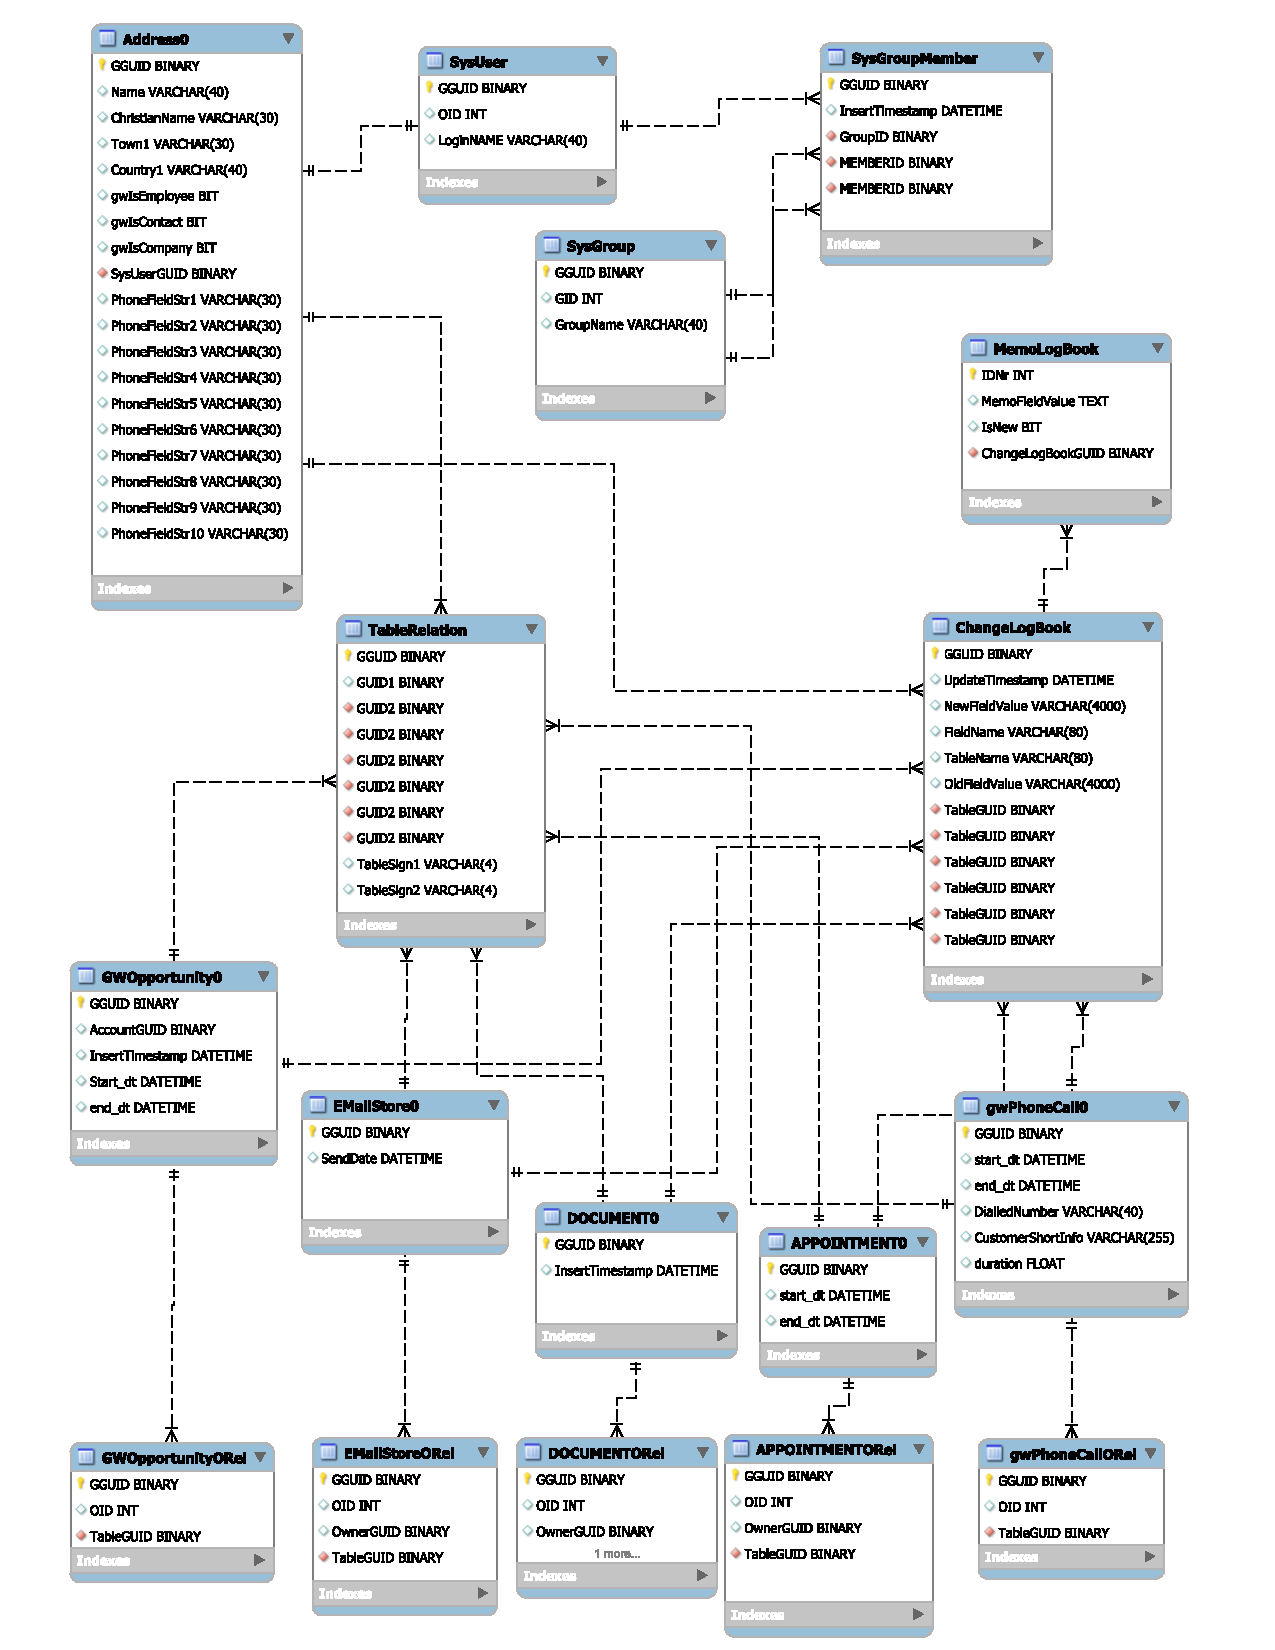
\includegraphics[width=1.0\textwidth]{pics/schema_alt.pdf}
	\caption{Auszug aus dem Schema der MSSQL-Datenbank}
	\label{gw_schema_alt}
\end{figure}

Die erste Tabelle \textit{SysUser} beinhaltet Informationen über Personen. Für die Umsetzung des Systems werden drei Attribute der Tabelle benötigt. Zum einen den Primärschlüssel der Tabelle, die \textit{GGUID}. Sie wird des Weiteren nicht mehr erwähnt, da sie in jeder Tabelle den Primärschlüssel darstellt. Das Attribut \textit{OID} wird in anderen Tabellen als Fremdschlüssel verwendet und wird somit zur Identifikation der jeweiligen Person benötigt. Das Attribut \textit{LoginName} repräsentiert den Benutzernamen der Personen und wird im neuen System weiterverwendet. 

Um Personen, die bestimmten Gruppen angehören, aus der Bewertung von Beziehungen auszuschließen werden die Tabellen \textit{SysGroupMember} und \textit{SysGroup} benötigt. Die erste der beiden Tabellen wird zur Realisierung der M:N-Beziehung zwischen \textit{SysUser} und \textit{SysGroup} verwendet. Sie beinhaltet neben den Fremdschlüsseln der andern Tabellen einen Zeitstempel. Dieser ermöglicht es nachzuvollziehen wann eine Person in eine Gruppe eingetreten ist. Der Zeitstempel wird zur Rekonstruktion von früheren Gruppenzusammensetzungen benötigt. Dadurch können die Personen ermittelt werden die zu einem Zeitpunkt in der Vergangenheit einer Gruppe angehörten oder auch nicht. Die Tabelle SysGroup enthält weiterhin die Attribute \textit{GroupName} und \textit{GID}. Ersteres beinhaltet den Namen einer Gruppe. Das andere Attribut wird benötigt, da es in anderen Tabellen als Fremdschlüssel verwendet wird.  

Weiterhin können Personen aus bestimmten Ländern oder Städten in der Bewertung nicht beachtet werden. Zu dessen Umsetzung wird die Tabelle \textit{Address0}  benötigt. Sie enthält die gesamte Anschrift der jeweiligen Personen allerdings werden nur die Attribute \textit{Town1} und \textit{Country1} verwendet. Neben der Anschrift wird in dieser Tabelle vermerkt ob eine Person ein Mitarbeiter, Firmenkontakt oder eine private Kontaktperson ist. Um diese Personen ausschließen zu können werden die Attribute \textit{gwIsEmployee}, \textit{gwIsCompany} und \textit{gwIsContact} benötigt. Weiterhin lässt sich mit der Tabelle feststellen welche Telefonnummern die entsprechende Person besitzt. Sie werden benötigt um die Telefongespräche zuordnen zu können. Die Attribute \textit{PhoneFieldStr1} bis \textit{PhoneFieldStr10} werden zur Aufbewahrung dieser Telefonnummern verwendet. 

Die Tabelle \textit{TableRelation} realisiert, wie in Abschnitt 3.1.3 behandelt, die M:N-Beziehungen zwischen allen Tabellen die CRM-Objekte repräsentieren. Sie wird benötigt um die CRM-Objekte einer Person zu ermitteln. Beispielsweise könnten alle von der Person erstellten Termine mit der \textit{GGUID} der Person ermittelt werden. Dafür müssen alle Tuppeln ermittelt werden dessen \textit{GUID1} mit der \textit{GGUID} der Person übereinstimmen. Infolgedessen sind mithilfe der Spalte \textit{GUID2} alle Fremdschlüssel der von der Person erstellten CRM-Objekte ersichtlich. Um nur die Termine zu erhalten sind ausschließlich Tupeln mit dem Kürzel "APP" in der Spalte \textit{TableSign2} zu berücksichtigen. 

Alle Informationen zu den Verkaufschancen finden sich in der Tabelle \textit{GWOpportunity0}. Das Attribut \textit{InsertTimestamp} wird zum Ermitteln des Erzeugungszeitpunktes benötigt. Die Attribute \textit{start\_dt} und \textit{end\_dt} geben den Zeitraum der Verkaufschance fest. Der betroffene Kunde der Verkaufschance kann über das Attribut AccountGUID ermittelt werden. Die Tabellen \textit{EmailStore0}, \textit{Document}, \textit{Appointment0} und \textit{gwPhoneCall0} enthalten die  Informationen der anderen vier CRM-Objekte. Eine Besonderheit in der  Tabelle \textit{EmailStore0} ist die Verwendung von \textit{SendDate} zur zeitlichen Einordnung einer E-Mail. Die Tabelle \textit{gwPhoneCall0} weist eine andere Besonderheit auf. Sie besitzt ein Attribut namens \textit{DialledNumber}, welches  zur Ermittlung des Gesprächspartners verwendet wird.  

Die Bewertung findet innerhalb von Zeiträumen statt. Dadurch müssen die Veränderungen von Daten über die Zeit hinweg beachtet werden. In der Datenbank werden sämtliche Aktualisierungen  der Datensätzen in der Tabelle \textit{ChangeLogBook} aufbewahrt. Sobald ein Feld in der Datenbank überschrieben wurde, wird eine neue Tupel in der \textit{ChangeLogBook} angelegt. In der Spalte \textit{UpdateTimestamp} wird der Zeitpunkt der Änderung erfasst. Die Spalte \textit{NewFieldValue} enthält den neuen Wert des geänderten Datensatzes. In der Spalte \textit{OldFieldValue} wird der alte Wert abgelegt. Mithilfe der Spalte \textit{TableName} ist nachvollziehbar in welcher Tabelle sich das geänderte Feld befindet und in \textit{FieldName} ist die Bezeichnung der betroffenen Spalte festgehalten. Um die Zeile in der die Änderung stattfand festzuhalten, wird die \textit{GGUID} der Tupel in der Spalte \textit{TableGUID} aufbewahrt. 

Einige Aktualisierungen in der Datenbank sind so umfangreich, dass die Änderungen die maximale Zeichenlänge des \textit{NewFieldValue} oder \textit{OldFieldValue} Attributs überschreitet. Damit diese Änderungen nicht verloren gehen wird die Tabelle \textit{MemoLogBook} eingesetzt. Sie besitzt ein Attribut namens\textit{MemoFieldFeld} vom Datentyp Text. Er ermöglicht es Zeichenfolgen in einer maximalen Länge von 536.870.911 Zeichen zu speichern. Dadurch können die Informationen abgespeichert werden, die zu groß für die Varchar-Felder aus der Tabelle \textit{ChangeLogBook} sind.     
